\documentclass[a4paper,12pt]{book}

\usepackage{url}
\usepackage[utf8x]{inputenc}
\usepackage{amsmath}
\usepackage{graphicx}
\graphicspath{{images/}}
\usepackage{hyperref}
\usepackage{enumitem}
\usepackage{fancyhdr}

\hypersetup{pdfborder = 0 0 0} %Remove box hyper refrence

\usepackage[svgnames]{xcolor} % Required for colour specification
\newcommand*{\plogo}{\fbox{$\mathcal{MB}$}} % Generic dummy publisher logo

\usepackage{tikz,lmodern}
\usepackage[most]{tcolorbox}

\usepackage{listings}

\definecolor{verde}{rgb}{0.25,0.5,0.35}
\definecolor{jpurple}{rgb}{0.5,0,0.35}
\definecolor{darkgreen}{rgb}{0.0, 0.2, 0.13}

\newcommand{\estiloJava}{
	\lstset{
		language=Java,
		basicstyle=\ttfamily\small,
		keywordstyle=\color{jpurple}\bfseries,
		stringstyle=\color{red},
		commentstyle=\color{verde},
		morecomment=[s][\color{blue}]{/**}{*/},
		extendedchars=true,
		showspaces=false,
		showstringspaces=false,
		numbers=left,
		numberstyle=\tiny,
		breaklines=true,
		backgroundcolor=\color{cyan!10},
		breakautoindent=true,
		captionpos=t,
		xleftmargin=0pt,
		tabsize=2
}}

\def\checkmark{\tikz\fill[scale=0.4](0,.35) -- (.25,0) -- (1,.7) -- (.25,.15) -- cycle;}

\usepackage[extrafootnotefeatures]{xepersian}
\settextfont[Scale=1.1]{B Nazanin}
\setlatintextfont[Scale=1]{Times New Roman}

%\linespread{1.3} %line spacing

% Header
\pagestyle{fancy}
% with this we ensure that the chapter and section
% headings are in lowercase.
\renewcommand{\chaptermark}[1]{%
	\markboth{#1}{}}
\renewcommand{\sectionmark}[1]{%
	\markright{\thesection\ #1}}
\fancyhf{} % delete current header and footer
\fancyhead[LE,RO]{\bfseries\thepage}
\fancyhead[LO]{\bfseries\rightmark}
\fancyhead[RE]{\bfseries\leftmark}
\renewcommand{\headrulewidth}{0.5pt}
\renewcommand{\footrulewidth}{0pt}
\addtolength{\headheight}{0.5pt} % space for the rule
\fancypagestyle{plain}{%
	\fancyhead{} % get rid of headers on plain pages
	\renewcommand{\headrulewidth}{0pt} % and the line
}

\begin{document}
	
	%----------------------------------------------------------------------------------------
	%	TITLE PAGE
	%----------------------------------------------------------------------------------------
	
	\begin{titlepage} % Suppresses headers and footers on the title page
		
		\centering % Centre all text
		
		%------------------------------------------------
		%	Title and subtitle
		%------------------------------------------------
		
		\setlength{\unitlength}{0.6\textwidth} % Set the width of the curly brackets above and below the titles
		
		{\color{LightGoldenrod}\resizebox*{\unitlength}{\baselineskip}{\rotatebox{90}{$\}$}}}\\[\baselineskip] % Top curly bracket
		
		\textcolor{Sienna}{\textit{\Huge \lr{Spring Cloud}}}\\[\baselineskip] % Title
		
		%{\color{RosyBrown}\Large }\\ % Subtitle or further description
		
		{\color{LightGoldenrod}\resizebox*{\unitlength}{\baselineskip}{\rotatebox{-90}{$\}$}}} % Bottom curly bracket
		
		\vfill % Whitespace between the title and the author name
		
		%------------------------------------------------
		%	Author
		%------------------------------------------------
		
		{\Large\lr{Milad Barzideh}}\\ % Author name
		
		\vfill % Whitespace between the author name and the publisher logo
		
		%------------------------------------------------
		%	Publisher
		%------------------------------------------------
		
		\plogo\\[0.5\baselineskip] % Publisher logo
		
		% Publisher name
		
	\end{titlepage}
	
	\tableofcontents
	
	%----------------------------------------------------------------------------------------
	%	Content
	%----------------------------------------------------------------------------------------
	
	\chapter{میکروسرویس‌ها، ابر و چیزهای دیگر}
	
	میکروسرویس‌‌  یا ریزخدمت\LTRfootnote{Microservice}
	یکی از اصطلاحاتی‌ست که این روزها در دنیای نرم‌افزار رایج شده است. میکروسرویس‌‌ها، سرویس‌هایی توزیع‌شده و مجزا هستند که هر کدام از آن‌ها وظیفه‌ی کوچک و مشخصی را انجام می‌دهند. در این نوشتار، پس از معرفی میکرسرویس‌ها و ذکر  مشخصه‌های آن،‌ با استفاده از فریمورک‌های 
	\lr{Spring Boot} 
	و
	\lr{Spring Cloud}
	به صورت عملی، معماری میکروسرویس‌ها را بررسی خواهیم کرد.
	
	\section{میکروسرویس چیست؟}
	قبل از مطرح شدن میکروسرویس‌ها بیشتر برنامه‌های تحت‌وب با استفاده از معماری یکپارچه\LTRfootnote{Monolithic}
	ساخته می‌شدند. در معماری یکپارچه، هر برنامه به عنوان یک محصول نرم‌افزاری قابل اجرا در نظر گرفته می‌شود و رابط کاربری، منطق برنامه و دسترسی به پایگاه داده همه در یک برنامه‌ی کاربردی قرار داده می‌شود. 
	
	هر برنامه به عنوان یک واحد کاری در نظر گرفته می‌شود که معمولا چندین تیم توسعه روی بخش‌های مختلف آن کار می‌کنند. یکی از مشکلاتی که در این حالت پیش می‌آید این است که با افزایش اندازه و پیچیدگی برنامه،‌ هزینه‌های ارتباطی و هماهنگی تیم‌ها، بیشتر و سخت‌تر می‌شود. برای مثال با هر تغییری که تیم‌ها ایجاد می‌کنند، کل برنامه  باید دوباره تست و مستقر\LTRfootnote{Redeployed} شود. 
	
	مفهوم میکروسرویس تقریبا از سال 2014 و در پاسخ به چالش‌هایی که برای مقیاس‌پذیر کردن برنامه‌های یکپارچه وجود داشت، وارد جامعه‌ی نرم‌افزار شد. همان‌طور که گفته شد یک میکروسرویس، کوچک، مجزا و توزیع‌شده است، بنابراین این امکان را فراهم می‌کند که برنامه‌های بزرگ را به بخش‌های کوچک‌تری تقسیم کرد تا مدیریت و توسعه‌ی آن‌ها آسان‌تر شود. مهم‌ترین نکته‌ای که باید به آن توجه داشت تجزیه و جداسازی عملکردهای برنامه است به صورتی که کاملا مستقل از همدیگر باشند. 
	
	\begin{figure}[h]
		\centering
		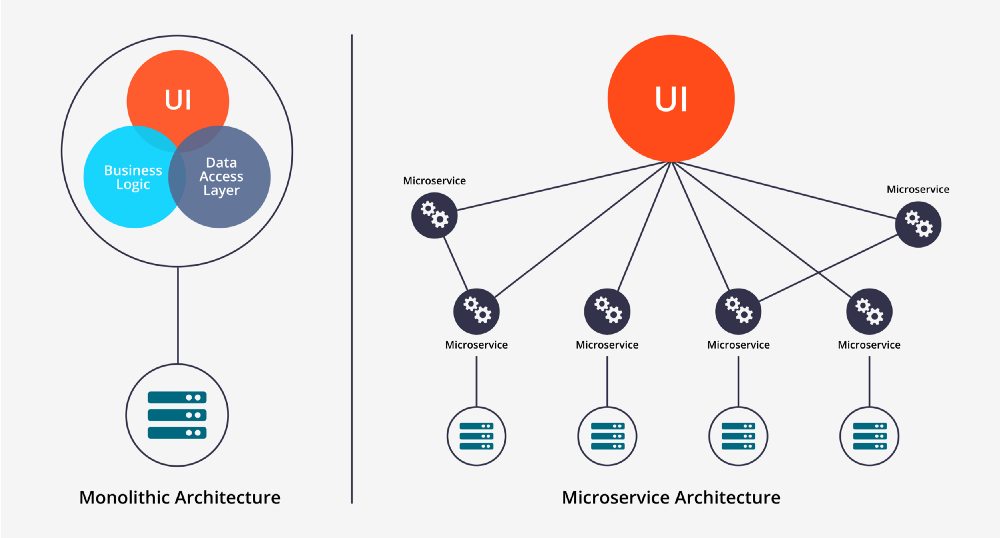
\includegraphics[width=\textwidth]{1.png}
		\caption{ معماری یکپارچه در مقابل معماری میکروسرویس}
		\label{fig:1}
	\end{figure}
	
	همان‌طور که شکل \ref{fig:1} نشان می‌دهد هر تیم می‌تواند کدها و زیرساخت مربوط به سرویس خود را داشته باشد و آن‌ها را به صورت مستقل نسبت‌ به سرویس‌های دیگر توسعه و ارزیابی کند.
	
	\vskip 0.2cm
	معماری میکروسرویس ویژگی‌های زیر را دارد:
	\begin{itemize}[label=$\ast$]
		\item  منطق برنامه به قسمت‌های کوچک‌تر شکسته می‌شود و هر قسمت مسئله‌ی مشخص و تعریف شده‌ای را حل می‌کند.
		\item هر قسمت مسئولیت مشخصی دارد و مستقل از سایر بخش‌ها توسعه و استقرار می‌یابد. همچنین میکروسرویس‌ها باید قابلیت استفاده‌ی مجدد در برنامه‌های دیگر را داشته باشند.
		\item میکروسرویس‌ها با استفاده از قواعد مشخص و بکارگیری پروتکل‌های ارتباطی سبک‌وزن\LTRfootnote{Lightweight} مانند \lr{HTTP} و 
		\lr{JSON}
		داده‌ها را مبادله می‌کنند.
		\item پیاده‌سازی فنی هر میکروسرویس بی‌اهمیت است؛ زیرا برنامه‌ها با پروتکل‌های مستقل از تکنولوژی\LTRfootnote{Technology-neutral protocol}
		با هم ارتباط برقرار می‌کنند. این یعنی برنامه‌‌ای که با معماری میکروسرویس ساخته شده می‌تواند از تکنولوژی‌ها و زبان‌های مختلفی استفاده کند. 
		\item میکروسرویس‌ها برای سازمان‌ها این امکان را فراهم می‌کنند که تیم‌های توسعه‌ی کوچک با وظایف کاری مشخص داشته باشند.
	\end{itemize} 
	
	
	\section{محاسبات ابری چیست؟}
	دنیای محاسبات به‌سرعت به‌ سمت توسعه‌ی نرم‌افزارهایی پیش می‌رود که به‌جای اجرا بر روی کامپیوترهای منفرد، به عنوان یک سرویس در دسترس میلیون‌ها مصرف‌کننده قرار داده می‌شوند. از این نظر، محاسبات ابری از دید کاربران نهایی ساختاری شبیه به یک توده‌ی ابر دارد که به واسطه‌ی آن می‌توانند به برنامه‌های کاربردی از هر جایی از دنیا دسترسی داشته باشند. 
	
	محاسبات ابری یک الگوی محاسباتی است که در آن تعداد بسیار زیادی از سیستم‌ها به صورت شبکه‌های خصوصی و یا عمومی به یکدیگر متصل شده‌اند تا زیرساخت پویا و مقیاس‌پذیری را برای برنامه‌های کاربردی، ذخیره داده‌ها و فایل‌ها فراهم آورند. با ظهور این تکنولوژی، هزینه‌ی محاسبات، میزبانی برنامه‌های کاربردی، ذخیره‌سازی محتوا و تحویل سرویس‌ها به طور قابل توجهی کاهش یافته است. ایده‌ی محاسبات ابری در اصل بر مبنای "استفاده مجدد از قابلیت‌های فناوری" است.
	
	\section{معماری لایه‌ای محاسبات ابری}
	رایانش ابری می‌تواند برای تحویل سرویس‌های موجود در لایه‌های مختلف، از سخت‌افزار گرفته تا برنامه‌ي کاربردی مورد استفاده قرار گیرد. در عمل ارائه‌دهندگان محاسبات ابری سرویس‌های مختلف آن را در سه گروه دسته‌بندی کرده‌اند: نرم‌افزار به عنوان سرویس\LTRfootnote{Software as a service}،
	پلتفرم به عنوان سرویس\LTRfootnote{Platform as a service}
	و زیرساخت به عنوان سرویس\LTRfootnote{Infrastructure as a service}.
	این گروه‌ها با همدیگر لایه‌های مختلف نمایش داده شده در شکل \ref{fig:11} را نشان می‌دهند.
	
	\begin{figure}[h]
		\centering
		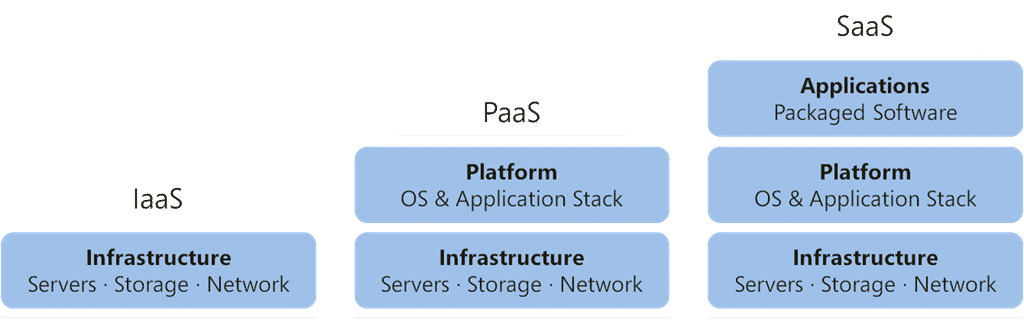
\includegraphics[width=\textwidth]{1-1.png}
		\caption{ لایه‌های مختلف محاسبات ابری}
		\label{fig:11}
	\end{figure} 
	
	
	\subsection{ نرم‌افزار به عنوان سرویس}
	نرم‌افزار به عنوان سرویس شامل یک برنامه‌ی کامل است که به‌صورت یک سرویس برحسب تقاضا فراهم می‌شود. یک نمونه‌ی واحد از نرم‌افزار روی ابر اجرا می‌شود و به چندین کاربر نهایی یا مشتری سازمانی سرویس می‌دهد.  
	
	\subsection{ پلتفرم به عنوان سرویس}
	پلتفرم  به عنوان سرویس یک لایه از نرم‌افزار را به صورت بسته‌بندی شده و به عنوان یک سرویس فراهم می‌کند به‌طوری که بتوان از آن برای ایجاد سرویس‌های سطح بالاتر استفاده کرد. 
	
	\subsection{ زیرساخت به عنوان سرویس}
	
	زیرساخت به عنوان سرویس، قابلیت‌های محاسباتی و ذخیره‌سازی اولیه را به عنوان سرویس‌های استاندارد در شبکه ارائه می‌دهد. سرورها، سیستم‌های ذخیره‌سازی، سوئیچ‌ها، روترها و دیگر سیستم‌ها با هم به عنوان مجموعه‌ای از منابع در دسترس هستند تا بار کاری و دیگر نیازمندی‌های برنامه‌های کاربردی که به توان بالایی نیاز دارند را مدیریت کنند. 
	
	\section{چرا ابر؟}
	
	به عنوان یک توسعه‌دهنده‌ی میکروسرویس، دیر یا زود باید تصمیم بگیرید سرویس‌تان را در یکی از مکان‌های زیر مستقر کنید:
	\begin{itemize}[label=$\ast$]
		\item \textit{سرور فیزیکی:} 
		سازمان‌های کمی این کار را انجام می‌دهند؛ زیرا سرورهای فیزیکی محدودیت ایجاد می‌کنند. برای مثال شما نمی‌توانید ظرفیت سرور فیزیکی را سریعا افزایش دهید یا یک میکروسرویس را به دلیل هزینه‌هایی زیادی که در پی دارد روی چندین سرور فیزیکی مستقر کنید.
		
		
		\item \textit{ماشین مجازی:}
		یکی از مهم‌ترین فواید میکروسرویس‌ها، توانایی آن‌ها در افزودن یا کاهش نمونه‌های یک سرویس است (مقیاس‌پذیری). یک میکروسرویس  را می‌توان در یک ماشین مجازی قرار داد و به آسانی چندین نمونه از آن را روی زیرساخت‌های موجود مستقر کرد.
		
		\item \textit{ظرف مجازی\LTRfootnote{Virtual container}:} 
		به جای استقرار میکروسرویس ‌روی یک ماشین مجازی کامل، بسیاری از توسعه‌دهندگان سرویس‌های خود را به صورت ظرف‌های داکر\LTRfootnote{Docker}
		در محیط ابری مستقر می‌کنند. 
	\end{itemize}
	
	
	\begin{tcolorbox}[colback=yellow!10!white,colframe=red!75!black,title=مطالعه‌ی بیشتر]
		
		\href{https://nickjanetakis.com/blog/comparing-virtual-machines-vs-docker-containers}
		{ تفاوت داکر با ماشین مجازی}
	\end{tcolorbox}
	
	\vskip 0.5cm
	مزیت مهم میکروسرویس‌های تحت ابر انعطاف‌پذیری بالای آن‌هاست. ارائه‌دهندگان محیط ابری اجازه می‌دهند در کم‌تر از چند دقیقه یک ماشین مجازی یا یک ظرف جدید را اضافه یا حذف کنید. همچنین برنامه‌ها مقاوم‌تر هستند، برای مثال اگر یکی از میکروسرویس‌ها از کار بیفتد می‌توان از نمونه‌های دیگر آن میکروسرویس استفاده کرد و برنامه را بالا نگه داشت. 
	
	
	
	
	
	
	
	
	
	
	
	\chapter{کنترل پیکربندی‌ها}
	به عنوان یک توسعه‌دهنده می‌دانید که
	\lr{hard-code} 
	کردن مقادیر در کدهای برنامه چندان منطقی نیست، به همین دلیل معمولا توسعه‌دهندگان از یک فایل ثابت استفاده می‌کنند و همه اطلاعات پیکربندی برنامه را در آن قرار می‌دهند. با این حال قرار دادن این اطلاعات در کدهای برنامه مشکل‌ساز است، زیرا با هر تغییر در پیکربندی، کل برنامه دوباره باید کامپایل شود. برای جلوگیری از این کار، توسعه‌دهندگان اطلاعات مربوط به پیکربندی را از کدهای برنامه جدا می‌کنند. 
	
	این مشکل در برنامه‌های تحت ابر بیشتر خود را نشان می‌دهد، از آن‌جا که ممکن است این برنامه‌ها از صدها میکروسرویس با چندین نمونه‌ی در حال اجرا تشکیل شده باشند، مدیریت پیکربندی برنامه بسیار مشکل است. برای همین توسعه‌ی میکروسرویس‌های تحت ابر روی موارد زیر تاکید دارد:
	\begin{enumerate}
		\item جداسازی پیکربندی برنامه از کدهای اصلی برنامه
		\item تزریق اطلاعات مربوط به پیکربندی برنامه در زمان راه‌اندازی سرور با استفاده از یک مخرن مرکزی به میکروسرویس‌‌های برنامه.
	\end{enumerate}
	
	
	\section{معماری مدیریت پیکربندی}
	
	همان‌طور که گفته شد لودشدن پیکربندی باید در راه‌‌اندازی\LTRfootnote{Bootstrapping} میکروسرویس‌ها انجام شود. 
	شکل \ref{fig:2} نقش مهم سرویس پیکربندی را برای راه‌اندازی میکروسرویس‌ها نشان می‌دهد:
	
	\begin{figure}[h]
		\centering
		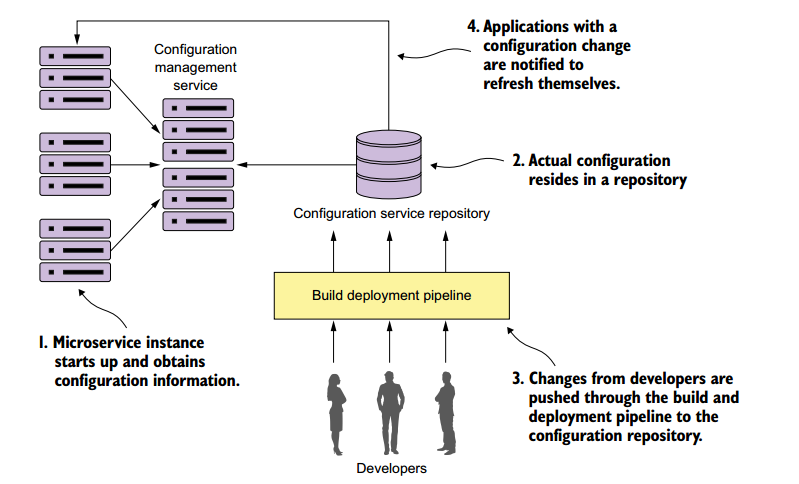
\includegraphics[width=\textwidth]{2.png}
		\caption{معماری مفهومی مدیریت پیکربندی‌ها}
		\label{fig:2}
	\end{figure}
	
	\begin{enumerate}
		\item
		قبل از اینکه یک نمونه از میکروسرویس بالا بیاید باید یک \lr{endpoint} را برای خواندن اطلاعات پیکربندی مربوط به خود صدا بزند. اطلاعات لازم برای فراخوانی \lr{endpoint} هنگام راه‌اندازی سرویس به آن پاس داده می‌شود.
		\item
		مخزن پیکربندی می‌تواند با استفاده از گیت، پایگاه‌داده‌های رابطه‌ای یا کلید-مقدار پیاده‌سازی شود.
		\item
		مدیریت داده‌های پیکربندی باید مستقل از چگونگی استقرار برنامه باشد.
		\item
		وقتی اطلاعات پیکربندی تغییر یابد؛ سرویس‌هایی که از آن اطلاعات استفاده می‌کنند باید از تغییر آگاه شوند و داده‌های خود را بروز کنند.
	\end{enumerate}
	
	
	
	\section{روش‌های پیاده‌سازی}
	برای پیاده‌سازی مدیریت پیکربندی پروژه‌های متن‌باز زیادی وجود دارد. شکل  \ref{fig:3}  برخی از آن‌ها را نشان می‌دهد.
	
	\begin{figure}[h]
		\centering
		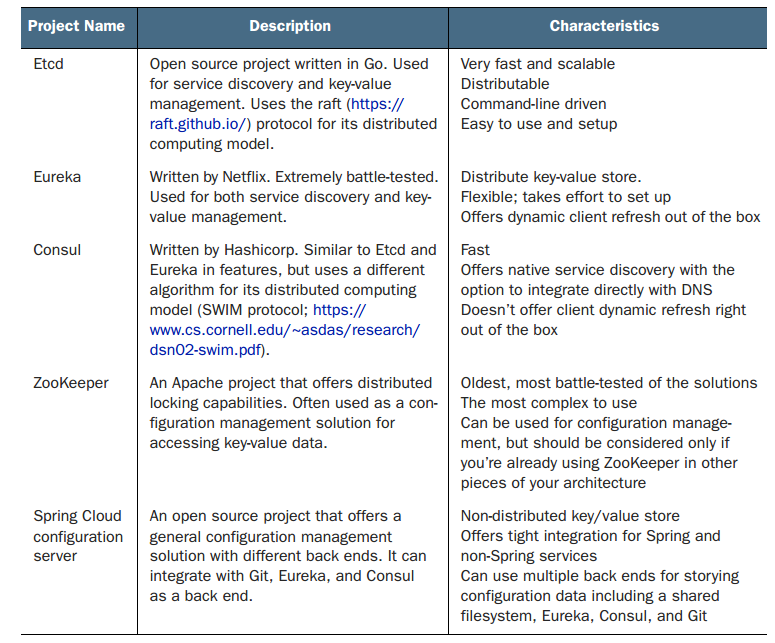
\includegraphics[width=\textwidth]{3.png}
		\caption{روش‌های پیاده‌سازی مدیریت پیکربندی}
		\label{fig:3}
	\end{figure}
	
	در اینجا از \lr{Spring Cloud configuration server} استفاده می‌شود. این روش نسبت به روش‌های دیگر ساده‌تر است، به خوبی  با \lr{Spring Boot}  ادغام می‌شود و از گزینه‌های بیشتری برای ذخیره داده‌های پیکربندی پشتیبانی می‌کند. 
	
	\section{پیاده‌سازی \lr{Spring Cloud configuration server}} 
	
	\lr{configuration server}
	یک برنامه‌ی \lr{REST-based} است که روی \lr{Spring Boot} ساخته می‌شود. کدهای \ref{lst:1}
	فایل \lr{pom.xml} را برای ساخت این سرویس نشان می‌دهند. 
	
	
	\begin{latin}
		\begin{scriptsize}
			\estiloJava
			\lstinputlisting[language=xml,firstline=0, lastline=56,caption= pom.xml, label=lst:1]{codes/config-server.xml}
		\end{scriptsize}
	\end{latin}
	
	در فایل \lr{Maven} بالا،‌ ابتدا نسخه‌ای از  \lr{Spring Boot} که در میکروسرویس‌ها از آن  استفاده می‌شود، مشخص شده است.  قسمت مهم بعدی  (خطوط 11-16) مشخص کردن نسخه‌ی \lr{Spring Cloud} است. \lr{Spring Cloud} شامل مجموعه‌ای از پروژه‌های مستقل است که هر کدام نسخه‌های مربوط به خود را دارند. با استفاده از این تعریف، تضمین می‌شود که از زیرپروژه‌های سازگار با هم در \lr{Spring Cloud} استفاده شود. قسمت بعدی مشخص کردن وابستگی‌های ...
		
		
		
		
		
	
	%\begin{tcolorbox}[colback=red!5!white,colframe=red!75!black]	
	%\end{tcolorbox}
	
\end{document}
